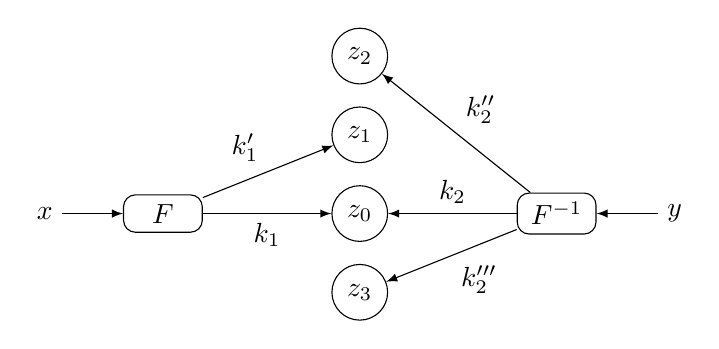
\begin{tikzpicture}
\node (x)  {$x$};
\node (f1) [right of=x, rounded corners=1ex, minimum width=1cm, draw,node distance = 1.5cm] {$F$};
\node (z) [right of=f1, circle, draw,node distance = 2.5cm] {$z_0$};
\node (f2) [right of=z, rounded corners=1ex, minimum width=1cm, draw,node distance = 2.5cm] {$F^{-1}$};
\node (y)  [right of=f2,node distance = 1.5cm] {$y$};
\node (z1) [above of=z, circle, draw] {$z_1$};
\node (z2) [above of=z1, circle, draw] {$z_2$};
\node (z3) [below of=z, circle, draw] {$z_3$};
\draw [-latex] (x)  -- (f1);
\draw [-latex] (f1) to node [auto,swap] {$k_1$} (z);
\draw [-latex] (f1) to node [auto] {$k_1'$} (z1);
\draw [-latex] (y) -- (f2);
\draw [-latex] (f2) to node [auto,swap] {$k_2$} (z);
\draw [-latex] (f2) to node [auto,swap] {$k_2''$} (z2);
\draw [-latex] (f2) to node [auto] {$k_2'''$} (z3);
\end{tikzpicture}